%% Direttive TeXworks:
% !TeX root = ../../maltoni_niccolo_tesi.tex
% !TEX encoding = UTF-8 Unicode
% !TEX program = arara
% !TEX TS-program = arara
% !TeX spellcheck = it-IT

%% Direttive Arara:
% arara: pdflatex: { shell: yes, synctex: yes, action: batchmode, options: "-halt-on-error -file-line-error-style" }
% arara: frontespizio
% arara: biber
% arara: pdflatex: { shell: yes, synctex: yes, action: batchmode, options: "-halt-on-error -file-line-error-style" }
% arara: pdflatex: { shell: yes, synctex: yes, action: nonstopmode, options: "-halt-on-error -file-line-error-style" }

\chapter{Conclusioni}\label{ch:conclusioni}
    \section{Risultati}\label{sec:risultati}
        L'obiettivo di questa tesi era quello di realizzare un'interfaccia grafica per l'ambiente di simulazione di Alchemist che sostituisse la precedente e si andasse ad integrare con i recenti contributi dati ad altre sezioni della GUI del software, andando a fornire una esperienza utente più semplice e gradevole anche per i meno esperti.

        L'interfaccia, realizzata con la libreria JavaFX, ha comportato un restyling completo a livello estetico e una reimplementazione di numerose parti del codice.
        Al termine del lavoro illustrato in questa tesi, essa risulta essere in grado di caricare una simulazione, rappresentarla a schermo attraverso effetti importabili ed esportabili per mezzo di file JSON e controllarne il flusso d'esecuzione; l'impatto sulle performance di simulazione rispetto a un'esecuzione \engEmph{headless} è accettabile e nei margini di quanto previsto.

        Di seguito è possibile vedere alcuni screenshot della GUI con una simulazione in esecuzione (\Crefrange{fig:simWithNodes}{fig:simWithDnD}).

        \begin{figure}[htbp]
            \centering
            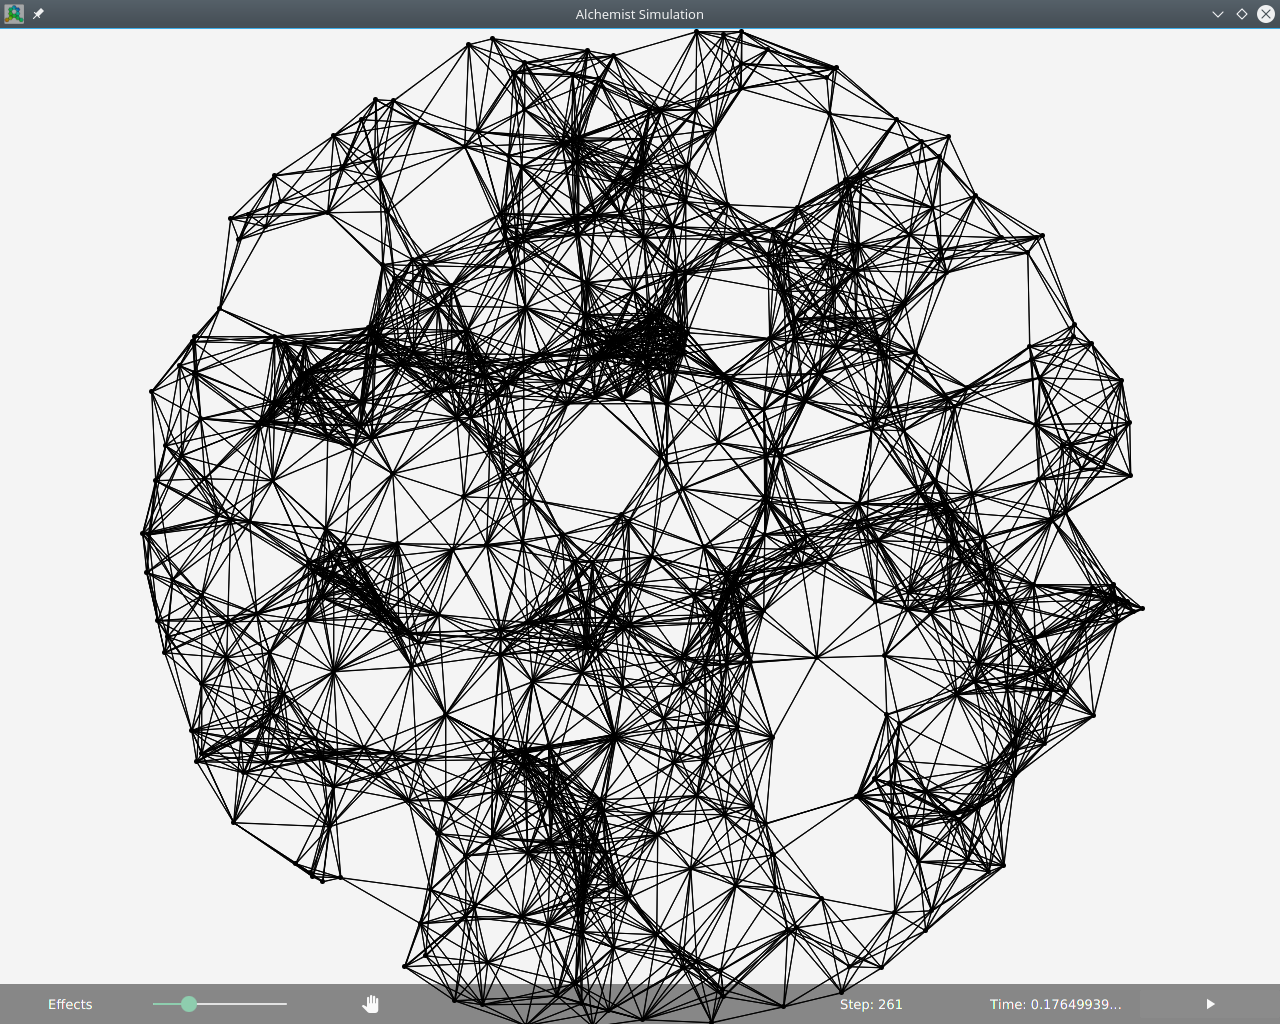
\includegraphics[scale=0.45]{img/withNodes/simWithNodes}
            \caption{Simulazione in corso di esecuzione}
            \label{fig:simWithNodes}
        \end{figure}

        \begin{figure}[htbp]
            \centering
            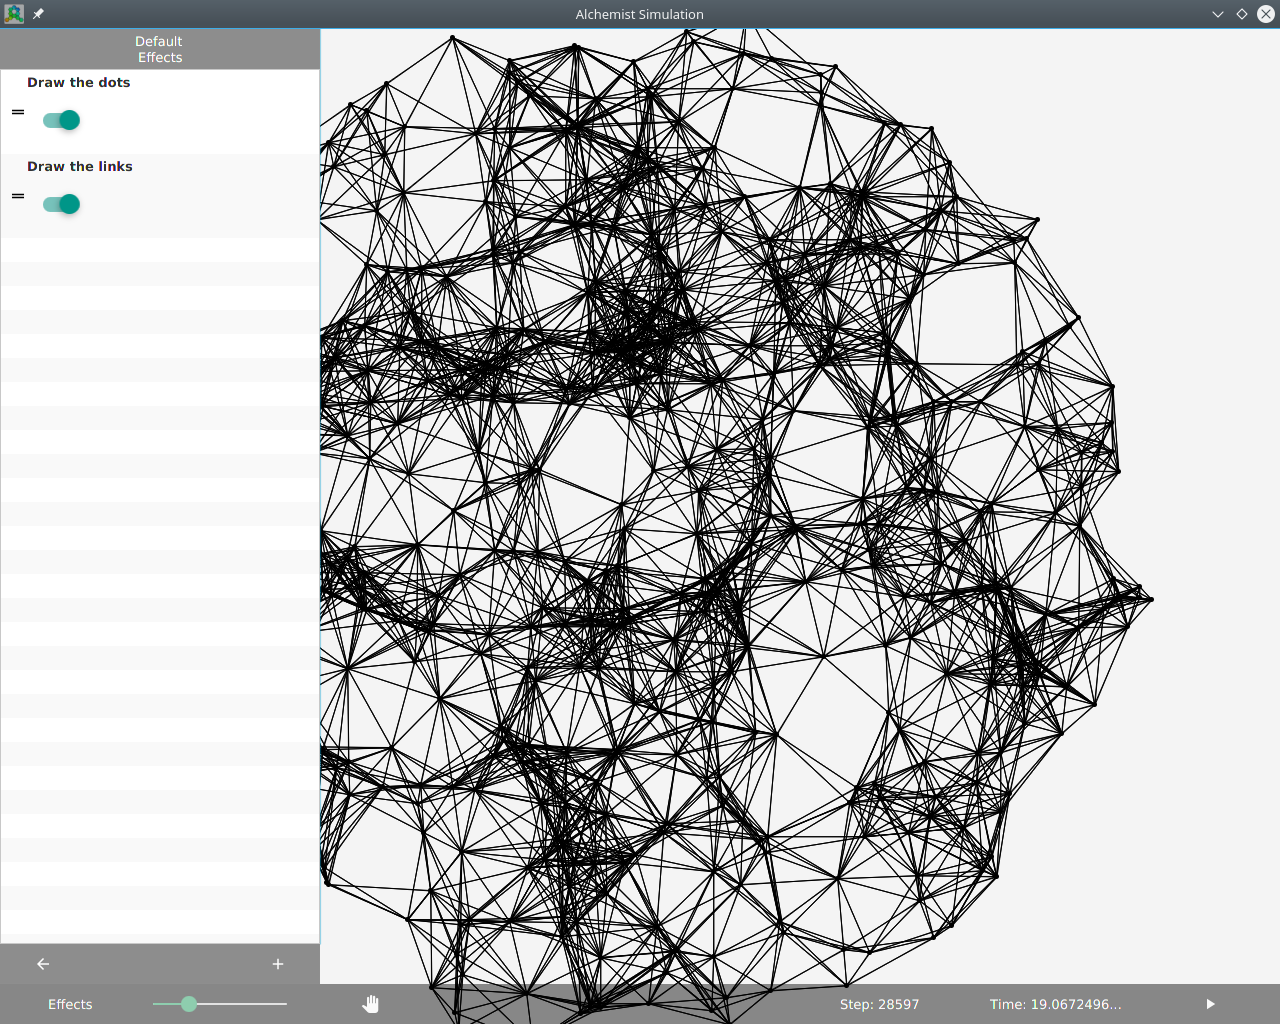
\includegraphics[scale=0.45]{img/withNodes/simWithEff}
            \caption{Drawer laterale degli effetti aperto}
            \label{fig:simWithEff}
        \end{figure}

        \begin{figure}[htbp]
            \centering
            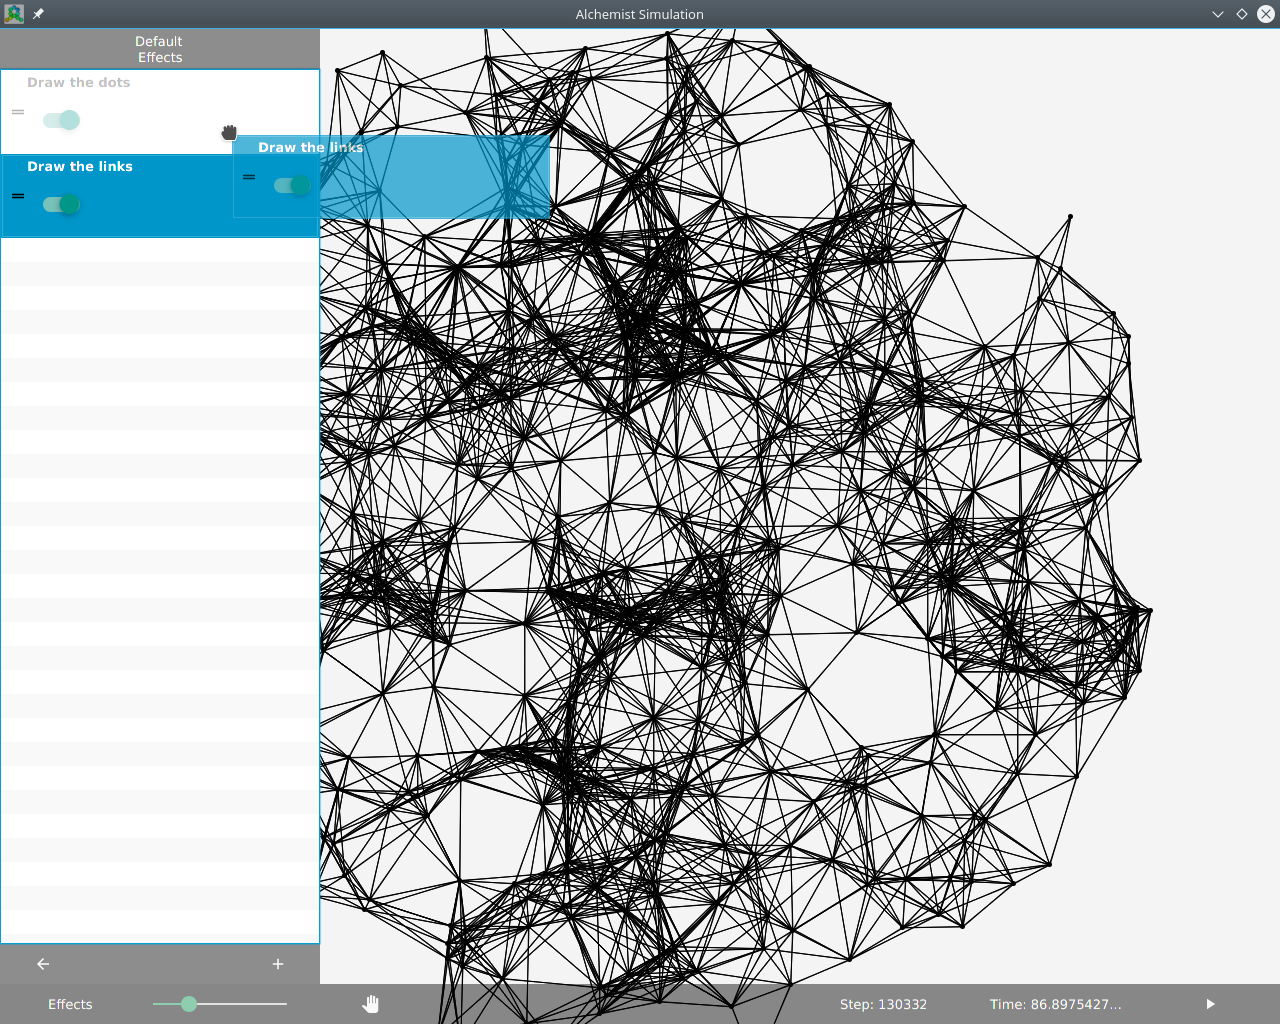
\includegraphics[scale=0.45]{img/withNodes/simWithDnD}
            \caption{Gestione \engEmph{Drag'n'Drop} degli effetti}
            \label{fig:simWithDnD}
        \end{figure}

        Nonostante il lavoro svolto sia funzionante, la mole di lavoro necessario non ha permesso di soddisfare tutti i requisiti e pertanto non può ancora sostituire completamente l'interfaccia classica. Nel paragrafo successivo sono illustrati i lavori futuri che possono essere apportati per rendere la GUI utilizzabile nel ramo stabile.

    \section{Lavori futuri}\label{sec:futuro}
        \textbf{\texttt{[...]}}
